The backend component integration should procede as described in the chapter 5.0.1, therefore it is unnecessary to repeat it in this section.
Despite this, the component integration between the frontend, the backend and all the other external service requires a deeper explanation by the following diagrams.
\section{Frontend-Backend application}
Firstly, the AuthorityWebApp requires a server on which it is to be hosted. Therefore, it will be deployed on the AuthorityWebServer component.
Also, the frontend components has to be integrated with the URIManager in order to ask for RESTful APIs, as described in the figure \ref{fig:frontend_urimanager_i_diagram}.
\begin{figure}[H]
    \centering
    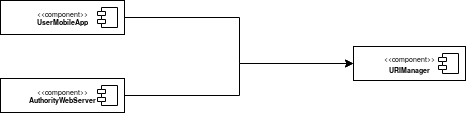
\includegraphics[width=.4\textwidth]{frontend_urimanager_i_diagram}
    \caption{Frontend-URIManager integration diagram}
    \label{fig:frontend_urimanager_i_diagram}
\end{figure}
On the other way, the Notification Service component has to be integrated with the respective frontend components, as described in fig. \ref{fig:notification_frontend_idiagram}
\begin{figure}[H]
    \centering
    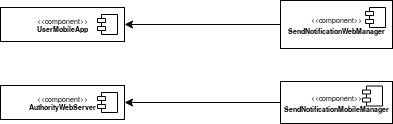
\includegraphics[width=.4\textwidth]{notification_frontend_idiagram}
    \caption{Notification-Frontend integration diagram}
    \label{fig:notification_frontend_idiagram}
\end{figure}
As far as the Cloud Database is concerned, the QueryManager has to be integrated with it as part of the data layer.
Finally, the external services have to be integrated with all the component that they require in order to perform their computation. The fig \ref{fig:external_services_idiagram} explains this matter in details.
\begin{figure}[H]
    \centering
    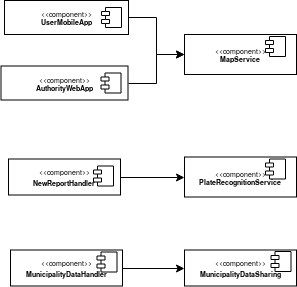
\includegraphics[width=.4\textwidth]{external_services_idiagram}
    \caption{External services integration diagram}
    \label{fig:external_services_idiagram}
\end{figure}